\documentclass[12pt,a4paper]{article}
\usepackage[utf8]{inputenc}
\usepackage[german]{babel}
\usepackage[T1]{fontenc}
\usepackage{times}
\usepackage{graphicx}
\usepackage{url}
\usepackage{color}
\usepackage{setspace}
\usepackage{enumerate}
\usepackage{amsmath}
\usepackage{amsfonts}
\usepackage{amssymb}
\usepackage{float}
\usepackage{stix}
\title{Zusammenfassung Rechnernetze}
\author{Henrik Tscherny}
\begin{document}
\maketitle
\tableofcontents
\section{Schichtenmodelle}
\textbf{Aufbau OSI-Schichtenmodell}\\
\begin{itemize}
\item Anwendungsschicht\\
Kommunikation zwischen Diensten (RPC, FTP, E-Mail, Telnet, WWW, ...)
\item Darstellungsschicht\\
Transformation zwischen Datenformaten, Kompression, Verschlüsselung (ASCII/EBCDIC, MPEG, MP3, RSA, ...)
\item Sitzungssicht\\
Kommunikations- und Dialogsteuerung, Synchronisation (simplex/duplex/halbduplex, Sicherungspunkte, Transaktionen)
\item Transportschicht\\
Sichere Ende-zu-Ende-Kommunikation zwischen Prozessen (Multiplex, Bündelung, Flusssteuerung)
\item Vermittlungsschicht\\
Wegewahl, Kopplung verschiedener Teilnetze (Anpassung, Abrechnung)
\item Sicherungsschicht\\
Rahmenbildung, Übertragungsfehlerbehandlung, Überlastvermeidung (Prüfsummen, Wiederholungen, Flusssteuerung)
\item Bitübertragungsschicht\\
Umsetzung in elektrische Signale, mechanische und elektrische Kopplung (RJ45-Stecker, ...)
\end{itemize}
Note: Oft werden die obersten 3 Sichten des OSI-Schichtenmodells als Anwendungsschicht zusammengefasst

\section{Formeln}
\begin{itemize}
\item B: Bandbreite in Hz
\item BR=SR: Baudrate, Signalschritte pro Sekunde in Baud (Bd)
\item b: Bitrate
\item S: Signalstufen
\item SNR: Signal-Rauschabstand
\item $f_g$ Grenzfrequenz
\item $f_a$ Abtastrate
\item QS: Quantisierungsstufen
\item $v_{phy}$: Ausbreitungsgeschwindigkeit (meist $\frac{2}{3}c$)
\item $\tau$: Signallaufzeit
\item SL: Start Limiter (Präambel + Start Frame Delimiter)
\item $t_f$: Übertragungsdauer
\item F: Framegröße
\item $BR=SR$
\item $b = SR \cdot ld(S)$
\item $SR = \frac{b}{ld(S)}$
\item $b < 2 \cdot B \cdot ld(S)$
\item $B > \frac{b}{2 \cdot ld(S)}$
\item $SNR_{db} = 10\cdot lg(SNR)$
\item $SNR = 10^{\frac{SNR_{db}}{10}}$
\item $b<B\cdot B \cdot ld(1+SNR)$
\item $B > \frac{b}{2 \cdot ld(1+SNR)}$
\item \textbf{Achtung! Immer schauen dass:}\\ $b<min\{2\cdot B \cdot ld(S), B \cdot ld(1+SNR)$
\item $f_a > 2 \cdot f_g$
\item $f_g > \frac{1}{2} f_a$
\item $f_a = \frac{b}{ld(QS)}$
\item $b = f_a \cdot ld(QS)$
\item $B_{gesammt} = n \cdot B_{kannal} + (n - 1) \cdot B_{abstand}$
\item $\tau = \frac{d}{v_{phy}}$
\item $t_s  = 2 \tau$
\item $t_f = \frac{SL+F}{b}$
\end{itemize}

\section{Bitübertragungsschicht}
\subsection{Modellierung}
\paragraph{Amplitudenmodulation}
\begin{itemize}
\item 0: niedrige Amplitude
\item 1: große Amplitude
\item geringster Aufwand aber kleinste Zuverlässigkeit 
\end{itemize}
\paragraph{Frequenzmodulation}
\begin{itemize}
\item 0: niedrige Frequenz (z.B. 1 Periode/Takt)
\item 1: hohe Frequenz	(z.B. 2 Perioden/Takt)
\item mittlerer Aufwand und mittlere Zuverlässigkeit
\end{itemize}
\paragraph{Phasenmodulation}
\begin{itemize}
\item 0: Phasensprung um $\phi=\pi$	(Signal bounced an x-Achse 1 Bogen auf der gleichen Seite weiter)
\item 1: kein Phasensprung
\item größter Aufwand aber höchste Zuverlässigkeit
\end{itemize}
\textbf{Quadrature Phase Shift Keying (QPSK)}\\
Nutzt Phasensprünge von $\phi \in \{ 0^\circ, 90^\circ ,180^\circ ,270^\circ\}$\\
Somit werden 2 Bit pro Signalschritt Kodiert\\
\\
\textbf{Quadrature Amplitude Modulation (QAM 16/ QAM 64)}\\
Nutzt 4/16 Phasensprünge d.h. 4/6 Bit pro Signalschritt\\

\subsection{Kodierung}
\subsubsection{Manchester-Kodierung}
\begin{itemize}
\item Non-Return-to-Zero (NRZI)
\item selbsttaktender Code
\item hoher Overhead 100\% (Netto = 0.5 Bitrate)
\item Pegeländerung in der Mitte jedes Taktes als Sync
\item 1: keine Pegeländerung an Intervallende
\item 0: Pegeländerung an Intervallende
\item eingesetzt bei Ethernet
\item Fehlererkennung auf Signalebene
\end{itemize}
\begin{figure}[H]
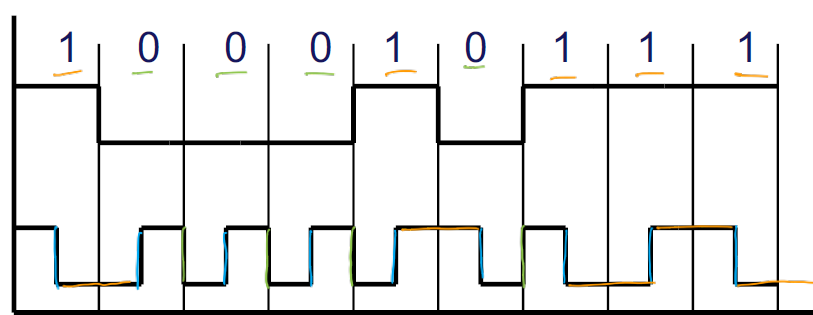
\includegraphics[scale=0.35]{./resources/manchester.png}
\end{figure}

\subsubsection{4B/5B-Code}
\begin{itemize}
\item erweitert Manchester Code
\item geringerer Overhead (25\%)
\item 4 Datenbits werden auf 5 Bits abgebildet
\item es dürfen nie mehr als 3 Nullen aufeinander folgen
\end{itemize}

\subsection{Multiplexing}
\begin{itemize}
\item Frequenzmultiplex: getrennte Frequenzbändern mit Sperrbändern dazwischen
\item orthogonales Frequenzmultiplex: Überlagerung verschiedener Frequenzbänder ohne Sperrbänder, benötigt FFT zur Trennung beim Empfänger
\item Zeitmultiplex: Teilnehmer erhalten zyklisch Sendezeit
\item statisches Zeitmultiplex: Feste Reihenfolge und Länge der Sendezeit für jeden Teilnehmer 
\item Codemultiplex (CDM): alle Teilnehmer senden zugleich aber mit verschiedener Kodierung
\item Wellenmultiplex (WDM): alle Teilnehmer senden zugleich aber über verschiedene Wellenlängen, benötigt Hardware zum Wiederauskoppeln
\end{itemize}

\section{Sicherungsschicht}
\paragraph{Carrierless Amplitude / Phase System}
Frequenzband wird statisch in für verschiedene Funktionen reserviert (z.B. up/download)\\
Trennung mit festen Schutzabständen
\paragraph{Discrete Multitone}
Aufteilung des Bandes in 247 Subbänder mit je 4kHz Breite\\
dynamisches Kombinieren und Zuteilen der Subbänder nach Bedarf

\subsection{ALOHA}
\begin{itemize}
\item Kommunikation erfolgt über Zentrale Station
\item Zwei Frequenzen für Hin- und Rückrichtung
\item Zentrale sendet Quittung zu Sender wenn erhalten
\item wenn keine Quittung eintrifft wird erneut gesendet
\item 18\% des Kanaldurchsatzes
\end{itemize}
\textbf{Sloted ALOHA}\\
\begin{itemize}
\item senden nur zu Beginn eines Taktes
\item 36\% des Kanaldurchsatzes
\end{itemize}

\subsection{Carrier Sense Multiple Access (CSMA)}
\begin{itemize}
\item Abhören des Kanals vor Sendevorgang\\
wenn kein Signal sende, sonnst warte
\item Trotzdem Kollision mögl. wenn beide gleichzeitig beginnen
\item nonpersistent CSMA: nicht sofortiges Erneutsenden sondern warten für eine zufällige Zeitspanne
\item p-persistent CSMA: Prüfe Kanal mit Wahrscheinlichkeit p sonnst warte einen Takt
\end{itemize}
\textbf{CSMA mit Collision Detection (CD)}
\begin{itemize}
\item Mithören auf Kanal während des Sendens
\item Dadurch schnelle Reaktion bei Kollision möglich (ohne warten auf Quittung)
\item Minimale Rahmenlänge für Sendevorgang $2 \tau$ mit $\tau$ = Signallaufzeit
\begin{itemize}
\item $t_0$ A Startet Übertragung
\item $t_0 + \tau - t_1$ B B Startet Übertragung bevor die von A eintrifft
\item $_0 + \tau$ Signal von A erreicht B -> Kollision wird von B erkannt
\item $t_0 + 2 \tau - t_1$ Signal von B erreicht A -> Kollision wird von A erkannt
\end{itemize}
\item Senden eines JAM-Signals bei erkannter Kollision an den Kommunikationspartner
\item NOTE: Heute werden alle möglichen Kollisionen im Switch behandelt wodurch CSMA/CD keine Rolle mehr spielt\\
zur Überlastkontrolle werden dabei PAUSE-Packete mit angegebener Wartezeit verwendet
\end{itemize}

\begin{figure}[H]
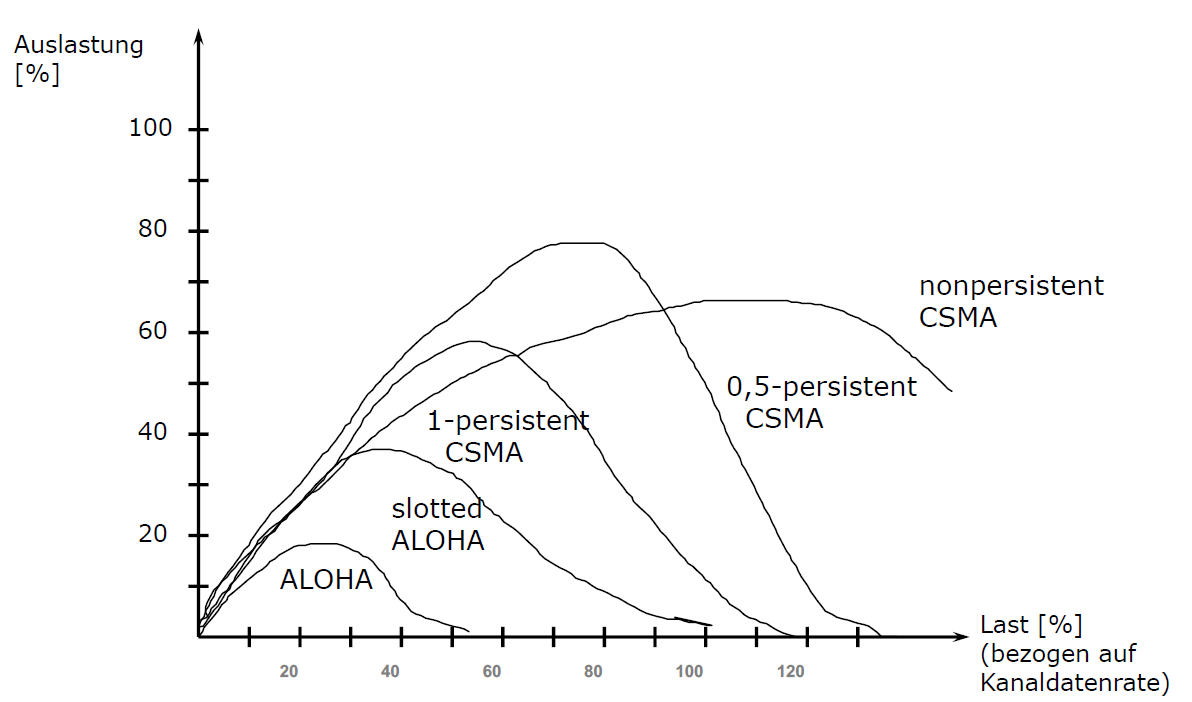
\includegraphics[scale=0.35]{./resources/durchsatz.png}
\end{figure}

\subsection{Switches}
\paragraph{Cut-Through Switches}
\begin{itemize}
\item Sofortiges Weiterleiten nach ermitteln der MAC-Adresse
\item Weiterleiten ohne Zwischenspeicherung
\item geringe Verzögerung
\item keine Fehlerkorrektur oder anpassen der Datenrate
\end{itemize}
\paragraph{Store-and-Forward Switches}

\begin{itemize}
\item Frames werden im Switch gepuffert
\item Frames können zwischenverarbeitet werden Fehlerkorrektur etc.
\item große Verzögerung
\end{itemize}
\paragraph{Adaptive Switching / Intelligent Switching}

\begin{itemize}
\item Arbeitet wie Cut-Through Switch aber speichert lokale Kopie der Frames
\item Überprüfung auf Fehler nach Weiterleitung
\item wenn zu viele Fehler auftreten wird in einen Store-and-Forward betrieb gewechselt
\end{itemize}
\paragraph{Fragment-free Switching}

\begin{itemize}
\item Packete werden auf Mindetgrößte überprüft
\item erkennen von Kollisionsüberresten
\end{itemize}

\subsection{Aufbau eines Ethernet-Frames}
\begin{figure}[H]
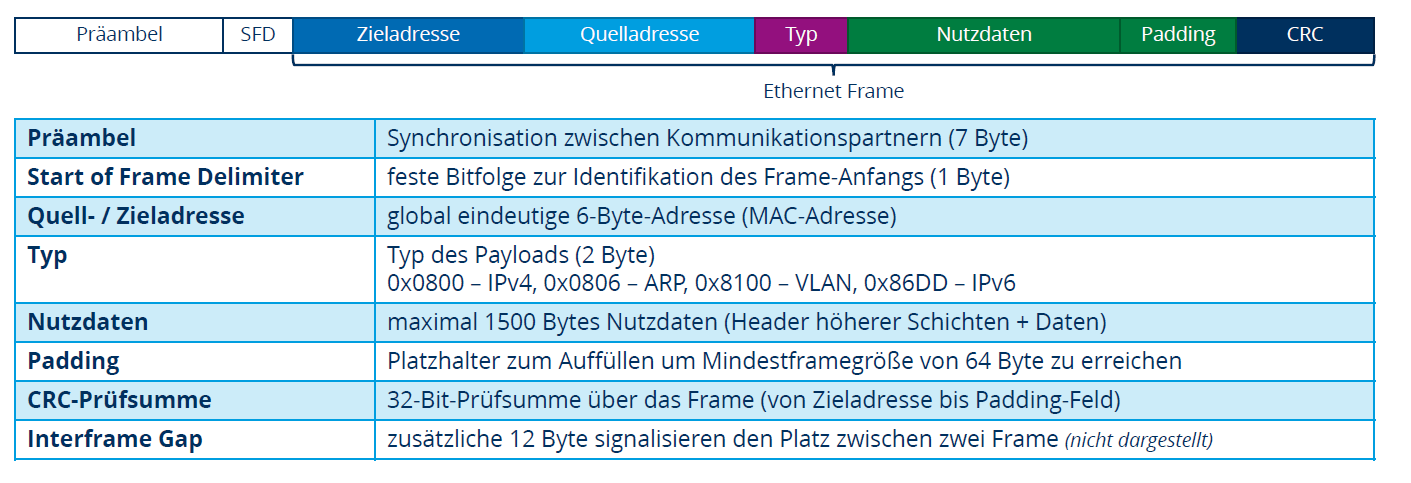
\includegraphics[scale=0.4]{./resources/ether-frame.png}
\end{figure}

\subsection{Frames/Rahmen}
\begin{itemize}
\item Bildet Einheit zur Datenübertragung / Fehlererkennung / Fehlerkorrektur
\item feingranulare Fehlerbehandlung
\item Steuerinformation mit Header und Trailer
\item Frames werden durch Frame Delimiter getrennt\\
-> Problem wenn FD (111111) 6x1 in Nutzdaten vorkommt
\begin{itemize}
\item 
\item Bitstuffing: Füge nach jeden aufeinanderfolgenden 5 Einsen im Payload eine 0 ein
\item Bytestuffing: Füge vor jeden im Payload auftretenden FD ein ESC-Byte ein, tritt ein ESC-Byte im Payload auf so füge davor auch ein ESC-Byte ein
\end{itemize}
\end{itemize}

\subsection{Fehlerkorrektur}
\paragraph{Hamming-Distanz}
\begin{itemize}
\item minimale Anzahl unterschiedlicher Bits zwischen 2 Quellwörtern
\item erkennbare Fehler: $d-1$
\item korrigierbare Fehler: $\lfloor\frac{d-1}{2}\rfloor$
\end{itemize}
\paragraph{Paritäts-Bit}
\begin{itemize}
\item Anhängen eines Bits an jede Bitfolge, sodass die Summe der Einsen gerade ist
\item Horizontale und Vertikale Paritätsbildung ermöglichen das Feststellen der genauen Fehlerstelle (wie in einer Matrix)
\end{itemize}
\paragraph{Cyclic Redundancy Check}
\begin{itemize}
\item $G(X)$: Generatorpolynom
\item $r$: Grad von $P_p$
\item $P_D$ : Datenpolynom
\item R: Rahmen (binäre Repräsentation von $P_D$
\item m: Anzahl der Bits im R (Grad von $P_D +1$)
\end{itemize}
\textbf{SENDEN}
\begin{itemize}
\item Hänge r Nullen an R an = $x^rP_D$
\item Teile $x^rP_D$ durch $G(X) mod 2$
\item Ziehe den Rest von $x^rP_D$ ab (XOR) = $P_S$
\item Fülle $P_S$ vorn mit Nullen auf den Grad von $G(X)$ auf
\item Sende Quellwort + $P_S$
\end{itemize}
\textbf{Empfangen}
\begin{itemize}
\item Teile $P_E$ durch $G(X) mod 2$
\item wenn Ergebnis = 0 Fehlerfreie Übertragung
\end{itemize}


\section{Vermittlungsschicht}
\paragraph{Shortest-Path-Routing}
\begin{itemize}
\item Dijkstra Algorithmus
\end{itemize}

\subsection{IP}
\begin{itemize}
\item identifiziert einen Host innerhalb eines Netzwerks
\item ein Host kann mehrere IP's haben
\end{itemize}

\begin{figure}[H]
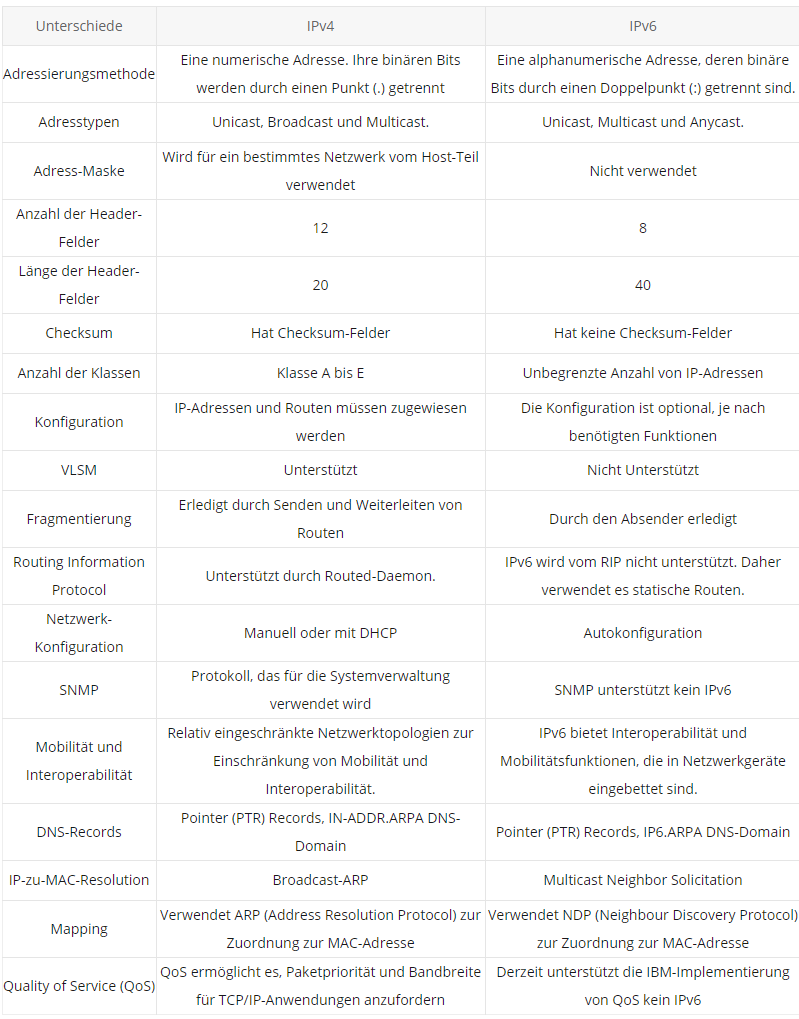
\includegraphics[scale=0.6]{./resources/v4v6.png}
\caption{Unterschied zwischen IPv4 und IPv6}
\end{figure}

\subsubsection{Subnetzmask}
\begin{itemize}
\item Jedes Subnetz erhält eine Netzadresse, welche aus dem ersten Teil (variable Länge) einer Hostadresse des Netzes gebildet wird
\item keine neuen Netzwerkadressen erforderlich
\item Subnetzadressen müssen außerhalb der Organisation nicht bekannt sein
\item Routingtabellen wird klein gehalten
\item CIDR Notation: IP/x wobei x der Subnetz-Anteil in Bits ist\\
Bsp: 192.168.0.1/24 -> 32-24 = 8 Host Bits -> [192.168.0.1 - 192.168.0.255]
\item gibt an welcher Teil der IP das Netz / den Host identifiziert
\item Anz. Hosts = $2^{32-CIDR} - \lfloor \frac{32-CIDR}{8} \rfloor$
\end{itemize}

\section{Transportschicht}
\

\end{document}